
\documentclass{article}
\usepackage{v-test-paper}

\begin{document}

\section*{PART ONE}
\subsection*{PHYSICAL FUNDAMENTALS OF MECHANICS}
\subsubsection*{KINEMATICS}

\begin{itemize}
  \item Average vectors of velocity and acceleration of a point:
  \begin{align*}
  \intertext{where $\Delta \mathbf{r}$ is the displacement vector (an increment of a radius vector).}
  \langle \mathbf{v} \rangle &= \frac{\Delta \mathbf{r}}{\Delta t}, \quad \langle \mathbf{w} \rangle = \frac{\Delta \mathbf{v}}{\Delta t}, \tag{1.1a}
  \end{align*}
  
  \item Velocity and acceleration of a point:
  \begin{align*}
  \mathbf{v} &= \frac{d\mathbf{r}}{dt}, \quad \mathbf{w} = \frac{d\mathbf{v}}{dt}. \tag{1.1b}
  \end{align*}
  
  \item Acceleration of a point expressed in projections on the tangent and the normal to a trajectory:
    \begin{align*}
    w_t &= \frac{dv_t}{dt}, \quad w_n = \frac{v^2}{R}, \tag{1.1c}
  \intertext{where $R$ is the radius of curvature of the trajectory at the given point.}
    \end{align*}
  
  \item Distance covered by a point:
  \begin{align*}
  s &= \int v dt, \tag{1.1d}
  \intertext{where $v$ is the modulus of the velocity vector of a point.}
  \end{align*}
  
  \item Angular velocity and angular acceleration of a solid body:
  \begin{align*}
  \boldsymbol{\omega} &= \frac{d\boldsymbol{\varphi}}{dt}, \quad \boldsymbol{\beta} = \frac{d\boldsymbol{\omega}}{dt}. \tag{1.1e}
  \end{align*}
  
  \item Relation between linear and angular quantities for a rotating solid body:
  \begin{align*}
  \mathbf{v} &= \boldsymbol{\omega} r, \quad w_n = \omega^2 R, \quad \lvert w_t \rvert = \beta R, \tag{1.1f}
  \intertext{where $\mathbf{r}$ is the radius vector of the considered point relative to an arbitrary point on the rotation axis, and $R$ is the distance from the rotation axis.}
  \end{align*}
  \end{itemize}

  \pagebreak
\begin{center}
  \textsc{Problems}
\end{center}
  \begin{enumerate}[label=1.\arabic*, start=1]
    
\item At time \( t = 0 \), terminal A in the circuit shown in the figure is connected to B by a key and an alternating current \( I(t) = I_0\cos(\omega t) \), with \( I_0 = 1 A \) and \( \omega = 500 \text{ rad s}^{-1} \) starts flowing in it with the initial direction shown in the figure. At \( t = \frac{7\pi}{6\omega} \), the key is switched from B to D. Now onwards only A and D are connected. A total charge \( Q \) flows from the battery to charge the capacitor fully. If \( C=20\mu F \), \( R=10 \Omega \) and the battery is ideal with \( emf \) of \( 50 V \), identify the correct statement(s).
    \begin{center}
        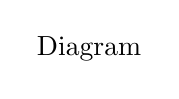
\begin{tikzpicture}
            \node at (0, 0) {Diagram};
        \end{tikzpicture}
    \end{center}
    \begin{tasks}(2)
        \task Magnitude of the maximum charge on the capacitor before \( t = \frac{7\pi}{6\omega} \) is \( 1 \times 10^{-3} C \).
        \task The current in the left part of the circuit just before \( t = \frac{7\pi}{6\omega} \) is clockwise.
        \task Immediately after A is connected to D, the current in \( R \) is \( 10 A \).
        \task \( Q = 2 \times 10^{-3} C \).
    \end{tasks}

    
\item A real gas behaves like an ideal gas if its
    \begin{tasks}(2)
        \task pressure and temperature are both high
        \task pressure and temperature are both low
        \task pressure is high and temperature is low
        \task pressure is low and temperature is high\ans
    \end{tasks}

    
\item A car starts moving rectilinearly, first with acceleration $w = -5.0\ m/s^2$ (the initial velocity is equal to zero), then uniformly, and finally, decelerating at the same rate $w$, comes to a stop. The total time of motion equals $\tau = 25\ s$. The average velocity during that time is equal to $\langle v \rangle = 72\ km$ per hour. How long does the car move uniformly?

    \item Given below are two statements:\\
\textbf{Statement I}: An elevator can go up or down with uniform speed when its weight is balanced with the tension of its cable.

\textbf{Statement II}: Force exerted by the floor of an elevator on the foot of a person standing on it is more than his/her weight when the elevator goes down with increasing speed.

In the light of the above statements, choose the correct answer from the options given below:
\begin{tasks}(1)
    \task Statement I is false but Statement II is true
    \task Both Statement I and Statement II are true
    \task Both Statement I and Statement II are false
    \task Statement I is true but Statement II is false
\end{tasks}
    
\item A point source $S$ is placed at the bottom of a transparent block of height $10\ mm$ and refractive index $2.72$. It is immersed in a lower refractive index liquid as shown in the figure. It is found that the light emerging from the block to the liquid forms a circular bright spot of diameter $11.54\ mm$ on the top of the block. The refractive index of the liquid is
    \begin{center}
        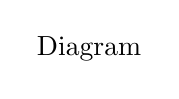
\begin{tikzpicture}
            \node at (0, 0) {Diagram};
            % Note: The actual diagram should replace this placeholder
        \end{tikzpicture}
    \end{center}
    \begin{tasks}(2)
        \task \(1.21\)
        \task \(1.30\)
        \task \(1.36\)
        \task \(1.42\)
    \end{tasks}

    
\item Consider a disc rotating in the horizontal plane with a constant angular speed $\omega$ about its centre $O$. The disc has a shaded region on one side of the diameter and an unshaded region on the other side as shown in the figure. When the disc is in the orientation as shown, two pebbles $P$ and $Q$ are simultaneously projected at an angle towards $R$. The velocity of projection is in the $y$-$z$ plane and is same for both pebbles with respect to the disc. Assume that (i) they land back on the disc before the disc has completed $\frac{1}{8}$ rotation, (ii) their range is less than half the disc radius, and (iii) $\omega$ remains constant throughout. Then
    \begin{center}
        
\begin{tikzpicture}
            \node at (0, 0) {diagram.png};
        \end{tikzpicture}
    \end{center}
    \begin{tasks}(1)
        \task $P$ lands in the shaded region and $Q$ in the unshaded region.
        \task $P$ lands in the unshaded region and $Q$ in the shaded region.
        \task Both $P$ and $Q$ land in the unshaded region.
        \task Both $P$ and $Q$ land in the shaded region.
    \end{tasks}

    \item Ratio of thermal energy released in two resistors \(R\) and \(3R\) connected in parallel in an electric circuit is :
\begin{tasks}(2)
    \task \(1 : 1\)
    \task \(1 : 27\)
    \task \(1 : 3\)
    \task \(3 : 1\)
\end{tasks}
    
\item A spherical metal shell A of radius $R_A$ and a solid metal sphere B of radius $R_B$ ($R_B < R_A$) are kept far apart and each is given charge $`+Q'$. Now they are connected by a thin metal wire. Then
    \begin{tasks}(2)
        \task $E_{\text{inside}}^A = 0$
        \task $Q_A > Q_B$
        \task $\frac{\sigma_A}{\sigma_B} = \frac{R_B}{R_A}$
        \task $E_{\text{on surface}}^A < E_{\text{on surface}}^B$
    \end{tasks}

    \item A bar of mass \( m \) is pulled by means of a thread up an inclined plane forming an angle \( \alpha \) with the horizontal (Fig. 1.13). The coefficient of friction is equal to \( k \). Find the angle \( \beta \) which the thread must form with the inclined plane for the tension of the thread to be minimum. What is it equal to?
    \begin{center}
        
\begin{tikzpicture}
            \node at (0, 0) {{image.png}};
        \end{tikzpicture}
    \end{center}
\begin{solution}
    \begin{center}
        \begin{tikzpicture}
            \pic at (0, 0) {frame=3cm};
        \end{tikzpicture}
    \end{center}
    
    \begin{align*}
        \intertext{Let us fix the $x - y$ co-ordinate system to the wedge, taking the $x$-axis up along the incline and the $y$-axis perpendicular to it (see figure).}
        \intertext{Now, we draw the free body diagram for the bar.}
        \intertext{Let us apply Newton’s second law in projection form along $x-$ and $y-$axes for the bar}
        T \cos \beta - mg \sin \alpha - fr &= 0 \tag{1}\\
        T \sin \beta + N - mg \cos \alpha &= 0 \tag{2}
        \intertext{or $N = mg \cos \alpha - T \sin \beta$}
        \intertext{But, $fr = kN$ and using Eq. (2) in Eq. (1), we get}
        T &= mg \sin \alpha + kmg \cos \alpha / (\cos \beta + k \sin \beta) \tag{3}
        \intertext{For $T_{\min}$ the value of $(\cos \beta + k \sin \beta)$ should be maximum}
        \frac{d (\cos \beta + k \sin \beta)}{d\beta} &= 0 \quad \text{or}\quad \tan \beta = k
        \intertext{Putting this value of $\beta$ in Eq. (3), we get}
        T_{\min} &= \dfrac{mg \left( \sin \alpha + k \cos \alpha \right)}{\sqrt{1+k^{2}}}
    \end{align*}
\end{solution}

    
\item Two bodies were thrown simultaneously from the same point: one, straight up, and the other, at an angle of $\theta = 60^\circ$ to the horizontal. The initial velocity of each body is equal to $v_0 = 25$ m/s. Neglecting the air drag, find the distance between the bodies $t = 1.70$ s later.

    
\item A point mass of \(1 \, \text{kg}\) collides elastically with a stationary point mass of \(5 \, \text{kg}\). After their collision, the \(1 \, \text{kg}\) mass reverses its direction and moves with a speed of \(2 \, \text{ms}^{-1}\). Which of the following statement(s) is (are) correct for the system of these two masses?
    \begin{tasks}(2)
        \task Total momentum of the system is \(3 \, \text{kg ms}^{-1}\)
        \task Momentum of \(5 \, \text{kg}\) mass after collision is \(4 \, \text{kg ms}^{-1}\)
        \task Kinetic energy of the centre of mass is \(0.75 \, \text{J}\)
        \task Total kinetic energy of the system is \(4 \, \text{J}\)
    \end{tasks}

    
\item In plotting stress versus strain curves for two materials \(P\) and \(Q\), a student by mistake puts strain on the \(y\)-axis and stress on the \(x\)-axis as shown in the figure. Then the correct statement(s) is(are)
        \begin{tasks}(2)
            \task \(P\) has more tensile strength than \(Q\)
            \task \(P\) is more ductile than \(Q\)
            \task \(P\) is more brittle than \(Q\)
            \task The Young's modulus of \(P\) is more than that of \(Q\)
        \end{tasks}
    \begin{center}
        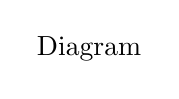
\begin{tikzpicture}
            \node {Diagram};
        \end{tikzpicture}
    \end{center}

    
\item A particle of mass \( M \) and positive charge \( Q \), moving with a constant velocity \( \vec{u}_1 = 4\hat{i} \, \text{ms}^{-1} \), enters a region of uniform static magnetic field normal to the \( xy \)-plane. The region of the magnetic field extends from \( x = 0 \) to \( x = L \) for all values of \( y \). After passing through this region, the particle emerges on the other side after 10 milliseconds with a velocity \( \vec{u}_2 = 2(\sqrt{3}\hat{i} + \hat{j}) \, \text{ms}^{-1} \). The correct statement(s) is (are)
    \begin{tasks}(2)
        \task The direction of the magnetic field is \(-z\) direction.
        \task The direction of the magnetic field is \(+z\) direction.
        \task The magnitude of the magnetic field is \( \frac{50 \pi M}{3Q} \) units.
        \task The magnitude of the magnetic field is \( \frac{100 \pi M}{3Q} \) units.
    \end{tasks}

    
\begin{enumerate}
    \item In the balanced condition, the values of the resistances of the four arms of a Wheatstone bridge are shown in the figure below. The resistance \( R_3 \) has temperature coefficient \( 0.0004 ^\circ C^{-1} \). If the temperature of \( R_3 \) is increased by \( 100^\circ C \), the voltage developed between \( S \) and \( T \) will be \_\_\_\_\_\_\_ volt.
    \begin{center}
        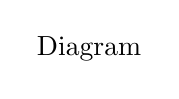
\begin{tikzpicture}
            \node {Diagram};
        \end{tikzpicture}
    \end{center}
\end{enumerate}

    
\item In the given circuit, the AC source has $\omega = 100\ \text{rad/s}$. Considering the inductor and capacitor to be ideal, the correct choice(s) is(are)
    \begin{center}
        \begin{circuitikz}[american]
            \draw (0,0)
            to[V, V=$20\ V$] (0,2) % The voltage source
            to[L, L=$0.5\ H$] (2,2) % The inductor
            to[C, C=$100\ \mu F$] (4,2) % The capacitor
            to[R, R=$100\ \Omega$] (4,0) % 100 ohm resistor
            -- (0,0);
            \draw (2,2)
            to[R, R=$50\ \Omega$] (2,0); % 50 ohm resistor
        \end{circuitikz}
    \end{center}
    \begin{tasks}(1)
        \task The current through the circuit, $I$ is $0.3\ A$.
        \task The current through the circuit, $I$ is $0.3\sqrt{2}\ A$.
        \task The voltage across $100\ \Omega$ resistor is $10\sqrt{2}\ V$.
        \task The voltage across $50\ \Omega$ resistor is $10\ V$.
    \end{tasks}

    \item A planet of mass \( M \), has two natural satellites with masses \( m_1 \) and \( m_2 \). The radii of their circular orbits are \( R_1 \) and \( R_2 \) respectively. Ignore the gravitational force between the satellites. Define \( v_1 \), \( L_1 \), \( K_1 \) and \( T_1 \) to be, respectively, the orbital speed, angular momentum, kinetic energy and time period of revolution of satellite 1; and \( v_2 \), \( L_2 \), \( K_2 \) and \( T_2 \) to be the corresponding quantities of satellite 2. Given \( m_1/m_2 = 2 \) and \( R_1/R_2 = 1/4 \), match the ratios in List-I to the numbers in List-II.

\begin{center}
    \renewcommand{\arraystretch}{2.5}
    \begin{table}
        \centering
        \begin{tabular}{p{0.25cm}p{6cm}|p{0.25cm}p{6cm}}
        \hline
        & List-I & &List-II \\
        \hline
        P. & \( \frac{v_1}{v_2} \) & 1. & \( \frac{1}{8} \) \\
        Q. & \( \frac{L_1}{L_2} \) & 2. & \( 1 \) \\
        R. & \( \frac{K_1}{K_2} \) & 3. & \( 2 \) \\
        S. & \( \frac{T_1}{T_2} \) & 4. & \( 8 \) \\
        \hline
        \end{tabular}
    \end{table}
\end{center}

\begin{tasks}(2)
    \task \( P \rightarrow 4; \) \( Q \rightarrow 2; \) \( R \rightarrow 1; \) \( S \rightarrow 3 \)
    \task \( P \rightarrow 3; \) \( Q \rightarrow 2; \) \( R \rightarrow 4; \) \( S \rightarrow 1 \)
    \task \( P \rightarrow 2; \) \( Q \rightarrow 3; \) \( R \rightarrow 1; \) \( S \rightarrow 4 \)
    \task \( P \rightarrow 2; \) \( Q \rightarrow 3; \) \( R \rightarrow 4; \) \( S \rightarrow 1 \)
\end{tasks}

\begin{solution}
    Since the satellites are in circular orbits, we can use the following equations governing their motion:
    \begin{align*}
        v &= \sqrt{\frac{GM}{R}} \quad \text{(Orbital speed)} \\
        L &= mRv \quad \text{(Angular momentum)} \\
        K &= \frac{1}{2}mv^2 \quad \text{(Kinetic energy)} \\
        T &= \frac{2\pi R}{v} \quad \text{(Time period)}
    \end{align*}
    where \( G \) is the gravitational constant.
    \begin{align*}
        \intertext{For the ratio \( P = \frac{v_1}{v_2} \), we use the orbital speed equation:}
        v_1 &= \sqrt{\frac{GM}{R_1}} \\
        v_2 &= \sqrt{\frac{GM}{R_2}} \\
        \frac{v_1}{v_2} &= \sqrt{\frac{R_2}{R_1}} = \sqrt{\frac{4}{1}} = 2 \quad \Rightarrow P \rightarrow 3.
        \intertext{For the ratio \( Q = \frac{L_1}{L_2} \), we use the angular momentum equation:}
        L_1 &= m_1R_1v_1 \\
        L_2 &= m_2R_2v_2 \\
        \frac{L_1}{L_2} &= \frac{m_1R_1}{m_2R_2}\frac{v_1}{v_2} = \frac{2}{1}\frac{1}{4}\cdot2 = \frac{1}{1} = 1 \quad \Rightarrow Q \rightarrow 2.
        \intertext{For the ratio \( R = \frac{K_1}{K_2} \), we use the kinetic energy equation:}
        K_1 &= \frac{1}{2}m_1v_1^2 \\
        K_2 &= \frac{1}{2}m_2v_2^2 \\
        \frac{K_1}{K_2} &= \frac{m_1}{m_2}\left(\frac{v_1}{v_2}\right)^2 = \frac{2}{1}\cdot2^2 = 8 \quad \Rightarrow R \rightarrow 4.
        \intertext{Finally, for the ratio \( S = \frac{T_1}{T_2} \), we use the time period equation:}
        T_1 &= \frac{2\pi R_1}{v_1} \\
        T_2 &= \frac{2\pi R_2}{v_2} \\
        \frac{T_1}{T_2} &= \frac{R_1}{R_2}\frac{v_2}{v_1} = \frac{1}{4}\cdot\frac{1}{2} = \frac{1}{8} \quad \Rightarrow S \rightarrow 1.
    \end{align*}
    Thus, we have P matching with 3, Q with 2, R with 4, and S with 1. The final answer is
    \begin{align*}
        P \rightarrow 3; \quad Q \rightarrow 2; \quad R \rightarrow 4; \quad S \rightarrow 1.\\
        \intertext{Therefore, option (b) is correct.}
    \end{align*}
\end{solution}
    \item Match List I with List II and select the correct answer using the codes given below the lists:

\begin{center}
    \renewcommand{\arraystretch}{2}
    \begin{table}[h]
        \centering
        \begin{tabular}{p{0.25cm}p{8cm}|p{0.25cm}p{5cm}}
        \hline
        & List I & & List II \\
        \hline
        (P)& Boltzmann constant & (1) & $[ML^2T^{-1}]$ \\
        (Q)& Coefficient of viscosity & (2) & $[ML^{-1}T^{-1}]$ \\
        (R)& Planck constant & (3) & $[MLT^{-3}K^{-1}]$ \\
        (S)& Thermal conductivity & (4) & $[ML^2T^{-2}K^{-1}]$ \\
        \hline
        \end{tabular}
    \end{table}
\end{center}

\begin{tasks}(2)
    \task $P \rightarrow 3$, $Q \rightarrow 1$, $R \rightarrow 2$, $S \rightarrow 4$
    \task $P \rightarrow 3$, $Q \rightarrow 2$, $R \rightarrow 1$, $S \rightarrow 4$
    \task $P \rightarrow 4$, $Q \rightarrow 2$, $R \rightarrow 1$, $S \rightarrow 3$
    \task $P \rightarrow 4$, $Q \rightarrow 1$, $R \rightarrow 2$, $S \rightarrow 3$
\end{tasks}
    
\begin{enumerate}
    \item A container with 1 kg of water in it is kept in sunlight, which causes the water to get warmer than the surroundings. The average energy per unit time per unit area received due to the sunlight is 700 Wm$^{-2}$ and it is absorbed by the water over an effective area of 0.05 m$^2$. Assuming that the heat loss from the water to the surroundings is governed by Newton’s law of cooling, the difference (in $^\circ$C) in the temperature of water and the surroundings after a long time will be \underline{\hspace{3cm}}. (Ignore effect of the container, and take constant for Newton’s law of cooling = 0.001 s$^{-1}$, Heat capacity of water = 4200 J kg$^{-1}$ K$^{-1}$)
\end{enumerate}

    
\item The focal length of a thin biconvex lens is \(20\text{cm}\). When an object is moved from a distance of \(25\text{cm}\) in front of it to \(50\text{cm}\), the magnification of its image changes from \(m_{25}\) to \(m_{50}\). The ratio \(\frac{m_{25}}{m_{50}}\) is \underline{\hspace{2.5cm}}.

    
\item An $\alpha$-particle and a proton are accelerated from rest by a potential difference of 100V. After this, their de Broglie wavelengths are $\lambda_\alpha$ and $\lambda_p$, respectively. The ratio $\frac{\lambda_p}{\lambda_\alpha}$, to the nearest integer, is \underline{\hspace{2.5cm}}.

    \item A horizontal plane supports a stationary vertical cylinder of radius \(R\) and a disc \(A\) attached to the cylinder by a horizontal thread \(AB\) of length \(l_0\) (Fig. 1.32, top view). An initial velocity \(v_0\) is imparted to the disc as shown in the figure. How long will it move along the plane until it strikes against the cylinder? The friction is assumed to be absent.
    \begin{center}
        \begin{tikzpicture}
            \node at (0, 0) {{diagram1.png}};
            \node[anchor=north] at (4, -2) {Fig. 1.33.};
        \end{tikzpicture}
    \end{center}
\begin{solution}
    \begin{center}
        \begin{tikzpicture}
            \pic at (0, 0) {frame=3cm};
        \end{tikzpicture}
    \end{center}

    \begin{align*}
        \intertext{Since the tension is always perpendicular to the velocity vector, the work done by the tension force will be zero. Hence, according to the work energy theorem, the kinetic energy or velocity of the disk will remain constant during it’s motion. Hence, the sought time \( t = \frac{s}{v_0} \), where \( s \) is the total distance traversed by the small disk during it’s motion.}
        \intertext{Now, at an arbitrary position (see figure)}
        ds &= (l_0 - R\theta) d\theta \\
        \intertext{So,}
        s &= \int\limits_{0}^{\frac{l_0}{R}} (l_0 - R\theta)d\theta \\
        \intertext{or}
        s &= \frac{l_0^2}{R} - \frac{Rl_0^2}{2R^2} = \frac{l_0^2}{2R} \\
        \intertext{Hence, the required time}
        t &= \frac{l_0^2}{2Rv_0}
        \intertext{Note: It should be clearly understood that the only uncompensated force acting on the disk A in this case is the tension T, of the thread. It is easy to see that there is no point here, relative to which the moment of force T is invariable in the process of motion. Hence conservation of angular momentum is not applicable here.}
    \end{align*}
\end{solution}

    \item As shown in the figure, in an experiment to determine Young’s modulus of a wire, the extension-load curve is plotted. The curve is a straight line passing through the origin and makes an angle of \(45^\circ\) with the load axis. The length of wire is 62.8cm and its diameter is 4mm. The Young’s modulus is found to be \(x \times 10^4 \text{Nm}^{-2}\). The value of \(x\) is \underline{\hspace{2.5cm}}.
    \begin{center}
        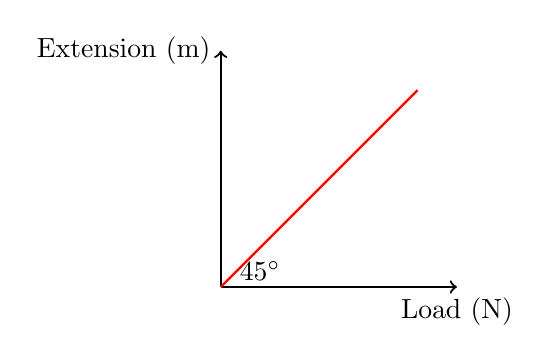
\begin{tikzpicture}
            \draw[->, thick] (0,0) -- (3,0) node[below] {Load (N)};
            \draw[->, thick] (0,0) -- (0,3) node[left] {Extension (m)};
            \draw[thick, red] (0,0) -- (2.5,2.5);
            \node at (0.5,0.2) {\(45^\circ\)};
        \end{tikzpicture}
    \end{center}
    \item Prism 1 of mass \(m_1\) and with angle \(\alpha\) (see Fig. 1.23) rests on a horizontal surface. Bar 2 of mass \(m_2\) is placed on the prism. Assuming the friction to be negligible, find the acceleration of the prism. 
    \begin{center}
        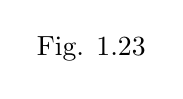
\begin{tikzpicture}
            \node at (0, 0) {Fig. 1.23};
        \end{tikzpicture}
    \end{center}
    \item Two cells are connected between points A and B as shown. Cell 1 has emf of 12 V and internal resistance of 3$\Omega$. Cell 2 has emf of 6V and internal resistance of 6$\Omega$. An external resistor R of 4$\Omega$ is connected across A and B. The current flowing through R will be \underline{\hspace{2.5cm}} A.
    \begin{center}
        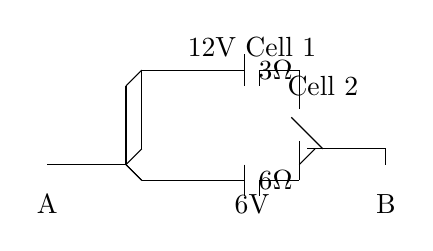
\begin{tikzpicture}
            \draw[-] (0,0) -- (1,0);
            \draw[-] (1,0) -- (1,1);
            \draw[-] (1,1) -- (1.2,1.2);
            \draw[-] (1,0) -- (1.2,-0.2);
            \draw[-] (1.2,1.2) -- (1.2,0.2);
            \draw[-] (1.2,0.2) -- (1,0);
            \draw[-] (1.2,-0.2) -- (1,0);
            \draw (1.2,1.2) -- (2,1.2);
            \draw (1.2,-0.2) -- (2,-0.2);
            
            % Cell 1
            \draw (2,1.2) -- (2.5,1.2);
            \draw (2.5,1.4) -- (2.5,1);
            \draw (2.7,1.2) -- (2.7,1);
            \node at (2.6,1.5) {12V Cell 1};
            \node at (2.9,1.2) {3$\Omega$};
            \draw (2.7,1.2) -- (3.2,1.2);
        
            % Cell 2
            \draw (2,-0.2) -- (2.5,-0.2);
            \draw (2.5,0) -- (2.5,-0.4);
            \draw (2.7,-0.2) -- (2.7,-0.4);
            \node at (2.6,-0.5) {6V};
            \node at (2.9,-0.2) {6$\Omega$};
            \draw (2.7,-0.2) -- (3.2,-0.2);
        
            % Connecting back to B
            \draw (3.2,1.2) -- (3.2,0.7);
            \draw (3.2,0.3) -- (3.2,-0.2);
            \draw (3.4,0.2) -- (3.2,0);
            \draw (3.1,0.6) -- (3.5,0.2);
            \draw (3.3,0.2) -- (4.3,0.2);
            \node at (3.5,1) {Cell 2};
            \draw (4.3,0.2) -- (4.3,0);
            
            % Points A and B
            \node (A) at (0,-0.5) {A};
            \node (B) at (4.3,-0.5) {B};
        \end{tikzpicture}
    \end{center}
    \item A hollow cylindrical conductor has length of 3.14 m, while its inner and outer diameters are 4 mm and 8 mm respectively. The resistance of the conductor is \( n \times 10^{-3} \Omega \). If the resistivity of the material is \( 2.4 \times 10^{-8} \Omega \text{m} \). The value of n is \underline{\hspace{2.5cm}}.

    \item A body of mass 1kg begins to move under the action of a time dependent force  $\vec{F} = \left( t\hat{i} +3t^{2}\hat{j} \right) N$, where $\hat{i}$ and $\hat{j}$ are the unit vectors along x and y axis. The power developed by above force, at the time $t = 2s$, will be \underline{\hspace{2.5cm}} W.
    \item Two simple harmonic waves having equal amplitudes of 8cm and equal frequency of 10Hz are moving along the same direction. The resultant amplitude is also 8cm. The phase difference between the individual waves is \underline{\hspace{2.5cm}} degree.
    \item A ball suspended by a thread swings in a vertical plane so that its acceleration values in the extreme and the lowest position are equal. Find the thread deflection angle in the extreme position.
\begin{solution}
    \begin{center}
        \begin{tikzpicture}
            \pic at (0, 0) {frame=3cm};
        \end{tikzpicture}
    \end{center}
    
    \begin{align*}
        \intertext{1.86 The ball has only normal acceleration at the lowest position and only tangential acceleration at either of the extreme positions, Let \( v \) be the speed of the ball at its lowest position and \( l \) be length of the thread, then according to the problem}
        \dfrac{v^2}{l} &= g \sin \alpha \tag{1} 
        \intertext{where \(\alpha\) is the maximum deflection angle.}
        \intertext{From Newton’s law in projection form: }
        F_t &= m v_t\\
        -mg \sin \theta &= m v \dfrac{dv}{l d\theta}\\
        -gl \sin \theta d\theta &= v dv
        \intertext{On integrating both the sides within their limits.}
        - gl \int_0^\alpha \sin \theta d\theta &= \int_v^0 v dv\\
        \intertext{or\quad \quad \quad \quad \( v^2 = 2gl (1 - \cos \alpha)\) \tag{2}}
        \intertext{Note: Eq. (2) can easily be obtained by the conservation of mechanical energy of the ball in the uniform field of gravity.}
        \intertext{From Eqs. (1) and (2) with \(\theta = \alpha\)}
        \sin \alpha &= 2 (1 - \cos \alpha)\\
        \sin \alpha + 2 \cos \alpha &= 2
        \intertext{On solving we get,}
        \alpha &\approx 53^\circ
    \end{align*}
\end{solution}

    \item The energy released per fission of nucleus of $^{240}X$ is 200 MeV. The energy released if all the atoms in 120g of pure $^{240}X$ undergo fission is \underline{\hspace{2.5cm}} $\times 10^{25}$ MeV.

    \begin{center}
        \begin{tikzpicture}
            \node at (0, 0) {};
        \end{tikzpicture}
    \end{center}
    \item As shown in the figure, three identical polaroids \( P_1 \), \( P_2 \), and \( P_3 \) are placed one after another. The pass axis of \( P_2 \) and \( P_3 \) are inclined at angle of \( 60^\circ \) and \( 90^\circ \) with respect to axis of \( P_1 \). The source S has an intensity of \( 256 \frac{W}{m^2} \). The intensity of light at point O is \underline{\hspace{2.5cm}} \( \frac{W}{m^2} \). 
    
    \begin{center}
        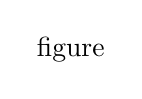
\begin{tikzpicture}
            \node at (0, 0) {{figure}};
        \end{tikzpicture}
    \end{center}
    \item A cyclist rides along the circumference of a circular horizontal plane of radius \(R\), the friction coefficient being dependent only on distance \(r\) from the centre \(O\) of the plane as \( k = k_0 (1 - r/R) \), where \( k_0 \) is a constant. Find the radius of the circle with the centre at the point along which the cyclist can ride with the maximum velocity. What is this velocity?
    \begin{center}
        
\begin{tikzpicture}
            \node at (0,0) {{cyclistdiagram.png}}; % Assume the diagram is saved as cyclist_diagram.png
        \end{tikzpicture}
    \end{center}

\begin{solution}
    \begin{center}
        \begin{tikzpicture}
            \pic at (0, 0) {frame=3cm};
        \end{tikzpicture}
    \end{center}
    
    \begin{align*}
        \intertext{According to the question, the cyclist moves along the circular path and the centripetal force is provided by the frictional force. Thus from the equation}
        F_n &= mw_n\\
        fr &= \dfrac{mv^2}{r} \quad \text{or} \quad kmg = \dfrac{mv^2}{r}\\
        k_0 \left( 1 - \dfrac{r}{R} \right) g &= \dfrac{v^2}{r} \quad \text{or} \quad v^2 = k_0 \left( r - \dfrac{r^2}{R} \right) g \tag{1}\\
        \intertext{For $v_{\text{max}}$ we should have}
        \dfrac{d}{dr} \left( r - \dfrac{r^2}{R} \right) &= 0\\
        1 - \dfrac{2r}{R} &= 0, \quad \text{so} \quad r = \dfrac{R}{2}\\
        \text{Hence,} \quad v_{\text{max}} &= \dfrac{1}{2} \sqrt{k_0 gR}
    \end{align*}
\end{solution}

    \item Two small discs of masses \( m_1 \) and \( m_2 \) interconnected by a weightless spring rest on a smooth horizontal plane. The discs are set in motion with initial velocities \( v_1 \) and \( v_2 \) whose directions are mutually perpendicular and lie in a horizontal plane. Find the total energy \( \mathcal{E} \) of this system in the frame of the centre of inertia.\begin{solution}
    \begin{align*}
        \intertext{As initially \(U = \tilde{U} = 0\), so, \(\tilde{E} = \tilde{T}\). From the solution of problem 1.147(b)}
        \tilde{T} &= \dfrac{1}{2} \mu |\vec{v}_1 - \vec{v}_2|\\
        \intertext{As}
        \vec{v}_1 &\perp \vec{v}_2\\
        \intertext{Thus,}
        \tilde{T} &= \dfrac{1}{2} \dfrac{m_1 m_2}{m_1 + m_2} (v_1^2 + v_2^2)
    \end{align*}
\end{solution}
    \item A car moves uniformly along a horizontal sine curve \( y = a \sin (x/\alpha) \), where \( a \) and \( \alpha \) are certain constants. The coefficient of friction between the wheels and the road is equal to \( k \). At what velocity will the car ride without sliding?
    
\item A balloon starts rising from the surface of the Earth. The ascension rate is constant and equal to \( v_0 \). Due to the wind the balloon gathers the horizontal velocity component \( v_x = ay \), where \( a \) is a constant and \( y \) is the height of ascent. Find how the following quantities depend on the height of ascent:
    \begin{enumerate}
        \item the horizontal drift of the balloon \( x(y) \);
        \item the total, tangential, and normal accelerations of the balloon.
    \end{enumerate}

    \item A fixed pulley carries a weightless thread with masses $m_{1}$ and $m_{2}$ at its ends. There is friction between the thread and the pulley. It is such that the thread starts slipping when the ratio $m_{2}/m_{1} = \eta_{0}$. Find:
    \begin{enumerate}
        \item the friction coefficient;
        \item the acceleration of the masses when $m_{2}/m_{1} = \eta > \eta_{0}$.
    \end{enumerate}
\begin{solution}
    \begin{center}
        \begin{tikzpicture}
            \pic at (0, 0) {frame=3cm};
        \end{tikzpicture}
    \end{center}
    
    \begin{align*}
        \intertext{Applying Newton's second law of motion in projection form, $F_n = mw_n$ for this element,}
        (T + dT) \sin (d\theta/2) + T \sin (d\theta/2) - dN &= dm\omega^2R = 0\\
        \intertext{or}
        2T \sin (d\theta/2) &= dN \quad [\text{neglecting the term } (dT \sin d\theta/2)]\\
        \intertext{or}
        T \, d\theta &= dN \left( \text{as } \sin \dfrac{d\theta}{2} \approx \dfrac{d\theta}{2} \right) \tag{1}\\
        \intertext{Also,}
        dfr &= kdN = (T + dT) - T = dT \tag{2}\\
        \intertext{From Eqs. (1) and (2)}
        kT \, d\theta &= dT \quad \text{or} \quad \dfrac{dT}{T} = kd\theta \\
        \intertext{Integrating $\theta \text{ from } 0 \text{ to } \theta = \pi$, we get}
        \ln \dfrac{T_2}{T_1} &= k\pi \tag{3}\\
        \intertext{So,}
        k &= \dfrac{1}{\pi} \ln \dfrac{T_2}{T_1} = \dfrac{1}{\pi} \ln \eta_0\\
        \left( \dfrac{T_2}{T_1} = \dfrac{m_2g}{m_1g} = \dfrac{m_2}{m_1} = \eta_0 \right)\\
        \intertext{When $m_2/m_1 = \eta > \eta_0$, the blocks will move with the same value of acceleration (say $w$) and clearly $m_2$ moves downward. From Newton's second law in projection form (downward for $m_2$ and upward for $m_1$), we get}
        m_2g - T_2 &= m_2w \tag{4}\\
        T_2 - m_1g &= m_1w \tag{5}\\
        \intertext{Also}
        \dfrac{T_2}{T_1} &= \eta_0 \tag{6}\\
        \intertext{Simultaneous solution of Eqs. (4), (5), and (6) yields}
        w &= \dfrac{(m_2 - \eta_0 m_1) g}{(m_2 + \eta_0 m_1)} = \dfrac{(\eta - \eta_0)}{(\eta + \eta_0)} g \quad \left( \dfrac{m_2}{m_1} = \eta \right)
    \end{align*}
\end{solution}

    \item A particle of mass \( m \) moves along the internal smooth surface of a vertical cylinder of radius \( R \). Find the force with which the particle acts on the cylinder wall if at the initial moment of time its velocity equals \( v_0 \) and forms an angle \( \alpha \) with the horizontal.
    \item Two identical buggies \( 1 \) and \( 2 \) with one man in each move without friction due to inertia along the parallel rails toward each other. When the buggies get opposite each other, the men exchange their places by jumping in the direction perpendicular to the motion direction. As a consequence, buggy \( 1 \) stops and buggy \( 2 \) keeps moving in the same direction, with its velocity becoming equal to \( v \). Find the initial velocities of the buggies \( v_1 \) and \( v_2 \) if the mass of each buggy (without a man) equals \( M \) and the mass of each man \( m \).
\begin{solution}
    \begin{center}
        \begin{tikzpicture}
            \pic at (0, 0) {frame=3cm};
        \end{tikzpicture}
    \end{center}
    
    \begin{align*}
        \intertext{Due to ejection of mass from a moving system (which moves due to inertia) in a direction perpendicular to it, the velocity of moving system does not change. The momentum change being adjusted by the forces on the rails. Hence in our problem velocities of buggies change only due to the entrance of the man coming from the other buggy. From conservation of linear momentum for the system (buggy 1 + man coming from buggy 2) in the direction of motion of buggy 1,}
        Mv_1 - mv_2 &= 0 \tag{1}\\
        \intertext{Similarly from conservation of linear momentum for the system (buggy 2 + man coming from buggy 1) in the direction of motion of buggy 2,}
        Mv_2 - mv_2 &= (M + m)v \tag{2}\\
        \intertext{Solving Eqs. (1) and (2), we get}
        v_1 &= \dfrac{mv}{M - m} \quad \text{and} \quad v_2 = \dfrac{Mv}{M - m}\\
        \intertext{As} 
        \vec{v_1} &\uparrow \downarrow \vec{v} \quad \text{and} \quad \vec{v_2} \uparrow \uparrow \vec{v}
        \intertext{So,}
        v_1 &= \dfrac{-mv}{M - m} \quad \text{and} \quad v_2 = \dfrac{Mv}{M - m}
    \end{align*}
\end{solution}

    \item A body of mass \( m \) is thrown at an angle to the horizontal with the initial velocity \( v_0 \). Assuming the air drag to be negligible, find:
    \begin{enumerate}
        \item the momentum increment \( \Delta p \) that the body acquires over the first \( t \) seconds of motion;
        \item the modulus of the momentum increment \( \Delta p \) during the total time of motion.
    \end{enumerate}
\begin{solution}
    \begin{align*}
        & \text{1.96} && \text{(a) We have} \\
        & \Delta \vec{p} \quad = \int_0^t \vec{F} dt = \int_0^t mg \, dt = mgt \quad \tag{1} \\
        & \text{(b) Using the solution of problem 1.28 (b), the total time of motion,} \\
        & \tau = -\dfrac{2 (\vec{v}_0 \cdot \vec{g})}{g^2} \\
        & \text{Hence, using } t = \tau \text{ in Eq. (1)} \\
        & |\Delta \vec{p}| = mg \, \tau \\
        & \quad \, = \dfrac{-2m (\vec{v}_0 \cdot \vec{g})}{g}
    \end{align*}
\end{solution}

    
\item A point moves along an arc of a circle of radius \( R \). Its velocity depends on the distance covered \( s \) as \( v = \alpha\sqrt{s} \), where \( \alpha \) is a constant. Find the angle \( \alpha \) between the vector of the total acceleration and the vector of velocity as a function of \( s \).

    
\item A particle moves along an arc of a circle of radius \( R \) according to the law \( l = a \sin \omega t \), where \( l \) is the displacement from the initial position measured along the arc, and \( a \) and \( \omega \) are constants. Assuming \( R = 1.00 \, m \), \( a = 0.80 \, m \), and \( \omega = 2.00 \, rad/s \), find:
    \begin{enumerate}
        \item the magnitude of the total acceleration of the particle at the points \( l = 0 \) and \( l = \pm a \);
        \item the minimum value of the total acceleration \( w_{\text{min}} \) and the corresponding displacement \( l_m \).
    \end{enumerate}

    \item A steel ball of mass $m = 50 \, \text{g}$ falls from the height $h = 1.0 \, \text{m}$ on the horizontal surface of a massive slab. Find the cumulative momentum that the ball imparts to the slab after numerous bounces, if every impact decreases the velocity of the ball $\eta = 1.25$ times.\begin{solution}
    \begin{center}
        \begin{tikzpicture}
            \pic at (0, 0) {frame=3cm};
        \end{tikzpicture}
    \end{center}
    
    \begin{align*}
        \intertext{Velocity of the ball, with which it hits the slab, \( v = \sqrt{2 gb} \).}
        \intertext{After first impact \( v' = ev \) (upward) but according to the problem}
        v' &= \dfrac{v}{\eta}, \quad \text{so} \quad e = \dfrac{1}{\eta}\\
        \intertext{and momentum imparted to this slab equals}
        mv &- (-mv') = mv (1 + e)\\
        \intertext{Similarly, velocity of the ball after second impact is}
        v'' &= ev' = e^2 v\\
        \intertext{and momentum imparted is}
        m(v' + v'') &= m(1 + e)ev\\
        \intertext{Again, momentum imparted during third impact is}
        m (1 + e)e^2v, \quad \text{and so on}
    \end{align*}
    
    \begin{align*}
        \intertext{Hence, net momentum imparted \(= mv (1 + e) + mve' (1 + e) + \cdots \)}
        &= mv(1 + e) (1 + e + e^2 + \cdots)\\
        &= mv \cdot \dfrac{(1+e)}{1 - e} \quad \text{(from summation of G.P.)}\\
        &= \sqrt{2 gb} \left( \dfrac{(1+1/\eta)}{1-1/\eta} \right)=m\sqrt{2 gb} \left( \dfrac{\eta + 1}{\eta - 1} \right) \quad \text{(using Eq. 1)}\\
        &= 0.2 \text{ kg m/s (on substituting values)}
    \end{align*}
\end{solution}
    \item A raft of mass $M$ with a man of mass $m$ aboard stays motionless on the surface of a lake. The man moves a distance $l$ relative to the raft with velocity $\vec{v}(t)$ and then stops. Assuming the water resistance to be negligible, find:
    \begin{enumerate}
        \item the displacement of the raft $l$ relative to the shore;
        \item the horizontal component of the force with which the man acted on the raft during the motion.
    \end{enumerate}
\begin{solution}
    \begin{center}
        \begin{tikzpicture}
            \pic at (0, 0) {frame=3cm};
        \end{tikzpicture}
    \end{center}

    \begin{align*}
        \intertext{Since the resistance of water is negligibly small the resultant of all external forces acting on the system “a man and a raft” is equal to zero. This means that the position of the C.M. of the given system does not change in the process of motion.}
        \vec{r}_C &= \text{constant} \quad \text{or} \quad \Delta \vec{r}_C = 0, \quad \sum m_i \Delta r_i = 0\\
        &\text{or} \quad m (\Delta r_{mM} + \Delta r_{Mp}) + M \Delta r_M  = 0\\
        &\text{Thus,} \quad m(l' + l) + M l = 0 \quad \text{or} \quad l = - \dfrac{ml'}{m + M}\\
        \intertext{(b) As net external force on “man-raft” system is equal to zero, therefore the momentum of this system does not change.}
        &\text{So,} \quad 0 = m[\vec{v}'(t) + \vec{v}_2(t)] + M \vec{v}_2(t)\\
        &\text{or} \quad \vec{v}_2(t) = - \dfrac{m \vec{v}'(t)}{m + M} \tag{1}\\
        &\text{Thus, the sought force on the raft}\\
        M \dfrac{d \vec{v}_2(t)}{dt} &= - \dfrac{Mm}{m + M} \dfrac{d \vec{v}'(t)}{dt}
        \intertext{Note: We may get the result of part (a), if we integrate Eq. (1) over the time of motion of man or raft.}
    \end{align*}
\end{solution}

    \item A stationary pulley carries a rope whose one end supports a ladder with a man and the other end the counterweight of mass \( M \). The man of mass \( m \) climbs up a distance \( l' \) with respect to the ladder and then stops. Neglecting the mass of the rope and the friction in the pulley axle, find the displacement \( l \) of the centre of inertia of this system.
\begin{solution}
    \begin{center}
        \begin{tikzpicture}
            \pic at (0, 0) {frame=3cm};
        \end{tikzpicture}
    \end{center}
    
    \begin{align*}
        \intertext{The displacement of the C.M. of the system, man $(m)$, ladder $(M - m)$ and the counterweight $(M)$, is described by radius vector}
        \Delta r_C &= \frac{\sum m_i \Delta r_i}{\sum m_i} = \frac{M \Delta r_M + (M - m) \Delta r_{(M-m)} + m \Delta r_m}{2M} \tag{1}\\
        \intertext{But,}
        \Delta r_m &= - \Delta r_{(M-m)}\\
        \intertext{and}
        \Delta r_m &= \Delta r_{m(M-m)} + \Delta r_{(M-m)} \tag{2}\\
        \intertext{Using Eq. (2) in Eq. (1) we get}
        \Delta r_C &= \frac{m l}{2M}
    \intertext{Alternate:}
    \intertext{Initially all the bodies of the system are at rest, and therefore the increments of linear momentum of the bodies in their motion are equal to the momentum themselves. The rope tension is the same both on the left and on the right-hand side, and consequently the momentum of the counter-balancing mass $(p_1)$ and the ladder with the man $(p_2)$ are equal at any instant of time, i.e., $p_1 = p_2$}
        M v_1 &= m v + (M - m) v_2\\
        \intertext{where $v_1,\;v,\; \text{and}\; v_2$ are the velocities of the mass, the man, and the ladder, respectively. Taking into account that $v_2 = -v_1 \; \text{and}\;v = v_2 + v'$, where $v'$ is the man's velocity relative to the ladder, we obtain}
        v_1 &= (m/2M) v'\\
        \intertext{On the other hand, the momentum of the whole system}
            p &= p_1 + p_2 = 2 p_1 \quad 2 M v_C = 2 M v_1 \tag{1}\\
        \intertext{where $V_C$ is the velocity of the centre of inertia of the system. With allowance made for Eq. (1) we get}
            V_C &= v_1 = (m/2M) v'\\
        \intertext{Finally, the sought displacement is}
        \Delta r_C &= \int V_C \, dt = (m/2M) \int v' \, dt = (m/2M) \Delta r'
    \end{align*}
\end{solution}

    \item A small bar starts sliding down an inclined plane forming an angle $\alpha$ with the horizontal. The friction coefficient depends on the distance $x$ covered as $k = ax$, where $a$ is a constant. Find the distance covered by the bar till it stops, and its maximum velocity over this distance.
    \item A body of mass \( m \) rests on a horizontal plane with the friction coefficient \( k \). At the moment \( t = 0 \) a horizontal force is applied to it, which varies with time as \( \mathbf{F} = at \), where \( a \) is a constant vector.
    \begin{enumerate}
        \item Find the distance traversed by the body during the first \( t \) seconds after the force action began.
    \end{enumerate}
    \item A body of mass \( m \) is thrown straight up with velocity \( v_0 \). Find the velocity \( v' \) with which the body comes down if the air drag equals \( kv^2 \), where \( k \) is a constant and \( v \) is the velocity of the body.\begin{solution}
    \begin{align*}
        \intertext{While going upward, from Newton’s second law, in vertical direction}
        m\dfrac{vdv}{ds} &= -(mg + kv^2)  \ \ \  \text{or}  \ \ \  \dfrac{vdv}{g + \left(kv^2 / m\right)} = -ds\\
        \intertext{At the maximum height \( h \), the speed \( v=0 \), so}
        \int_{v_0}^{0} \dfrac{vdv}{g + \left(kv^2 / m\right)} &= -\int_{0}^{b} ds\\
        \intertext{Integrating and solving, we get}
        h &= \dfrac{m}{2k} \ln{\left(1 +  \dfrac{kv_0^2}{mg} \right)}  \tag{1}\\
        \intertext{When the body falls downward, the net force acting on the body in downward direction equals \( mg - kv^2 \). Hence net acceleration, in downward direction, according to second law of motion}
        \dfrac{vdv}{ds} &= g - \dfrac{kv^2}{m}  \ \ \ \ \text{or} \ \ \  \dfrac{vdv}{g - \left(kv^2 / m\right)} = ds\\
        Thus, \int_{0}^{v'} \dfrac{vdv}{g - \left(kv^2 / m\right)} &= \int_{0}^{b} ds\\\
        \intertext{Integrating and putting the value of \textit{h} from Eq. \((1)\), we get}
        v' &= \dfrac{v_0}{\sqrt{1 + \dfrac{kv_0'^2}{mg}}}
    \end{align*}
\end{solution}
    \item A particle of mass \( m \) moves in a certain plane \( P \) due to a force \( F \) whose magnitude is constant and whose vector rotates in that plane with a constant angular velocity \( \omega \). Assuming the particle to be stationary at the moment \( t = 0 \), find:
    \begin{center}
        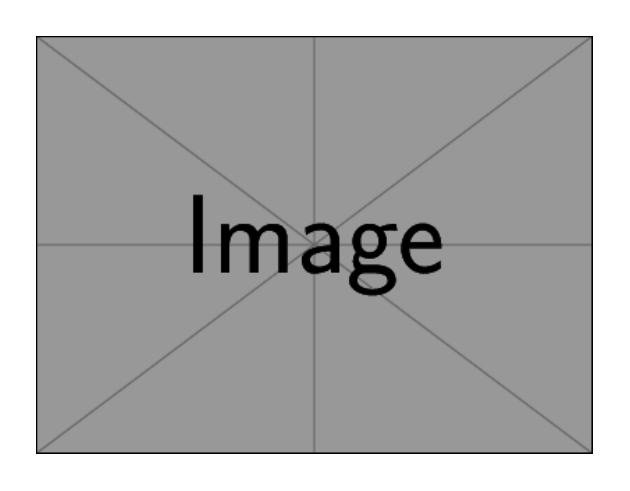
\begin{tikzpicture}
            \node at (0, 0) {\includegraphics[scale=0.5]{example-image.png}};
        \end{tikzpicture}
    \end{center}
    \begin{enumerate}
        \item its velocity as a function of time;
        \item the distance covered by the particle between two successive stops, and the mean velocity over this time.
    \end{enumerate}
    
\item A solid body rotates with deceleration about a stationary axis with an angular deceleration \(\beta \propto \sqrt{\omega}\), where \(\omega\) is its angular velocity. Find the mean angular velocity of the body averaged over the whole time of rotation if at the initial moment of time its angular velocity was equal to \(\omega_0\).

\begin{solution}
    \begin{align*}
        \intertext{In accordance with the problem, $\beta_x < 0$.}
        \text{Thus} \quad -\dfrac{d\omega}{dt} &= k \sqrt{\omega} \quad (\text{where } k \text{ is proportionality constant})\\
        \text{or} \quad -\int_{\omega_0}^{\omega} \dfrac{d\omega}{\sqrt{\omega}} &= k \int_{0}^{t} dt \quad \text{or} \quad \sqrt{\omega} = \sqrt{\omega_0} - \dfrac{kt}{2} \tag{1}\\
        \intertext{When \(\omega = 0\), total time of rotation \(t = \tau = \dfrac{2\sqrt{\omega_0}}{k}\)}
        \text{Average angular velocity} \quad <\omega> &= \dfrac{\int_{0}^{t} \omega \, dt}{\int_{0}^{t} dt} = \dfrac{\int_{0}^{2\sqrt{\omega_0}/k} \left(\omega_0 + \dfrac{k^2 t^2}{4} - kt \sqrt{\omega_0}\right) dt}{2\sqrt{\omega_0}/k}\\
        &= \dfrac{\left[ \omega_0 t + \dfrac{k^2 t^3}{12} - \dfrac{k}{2} \sqrt{\omega_0} t^2 \right]_0^{2\sqrt{\omega_0}/k}}{2\sqrt{\omega_0}/k}\\
        \intertext{Hence,}
        <\omega> &= \dfrac{\omega_0}{3}
    \end{align*}
\end{solution}

    \item A solid body rotates about a stationary axis so that its angular velocity depends on the rotation angle $\varphi$ as $\omega = \omega_0 - a\varphi$, where $\omega_0$ and $a$ are positive constants. At the moment $t = 0$ the angle $\varphi = 0$. Find the time dependence of
    \begin{enumerate}
        \item the rotation angle;
        \item the angular velocity.
    \end{enumerate}
    
\item A solid body starts rotating about a stationary axis with an angular acceleration \(\beta = \beta_0 \cos \varphi\), where \(\beta_0\) is a constant vector and \(\varphi\) is an angle of rotation from the initial position. Find the angular velocity of the body as a function of the angle \(\varphi\). Draw the plot of this dependence.

    
\item A rotating disc (Fig. 1.6) moves in the positive direction of the x axis. Find the equation \( y(x) \) describing the position of the instantaneous axis of rotation, if at the initial moment the axis \( C \) of the disc was located at the point \( O \) after which it moved
    \begin{enumerate}
        \item with a constant velocity \( v \), while the disc started rotating counterclockwise with a constant angular acceleration \( \beta \) (the initial angular velocity is equal to zero);
    
        \item with a constant acceleration \( w \) (and the zero initial velocity), while the disc rotates counterclockwise with a constant angular velocity \( \omega \).
    \end{enumerate}

\begin{solution}
    \begin{center}
        \begin{tikzpicture}
            \pic at (0, 0) {frame=3cm};
        \end{tikzpicture}
    \end{center}
    
    \begin{align*}
        \intertext{Therefore the velocity vector of an arbitrary point \( P \) of the solid can be represented as:}
        \vec{v}_P &= \vec{w} \times r_{PI} = \vec{w} \times \rho_{PI} \tag{1}
        \intertext{(where \( \rho_{PI} \) is normal location of point \( P \) relative to instantaneous rotation axis passing through point \( I \).)}
        \intertext{So instantaneous rotation axis  \( I \) is at the perpendicular distance \( \rho_{PI} = v_P / \omega \) from point \( P \).}
        \intertext{On the basis of Eq.~(1) for the centre of mass (C.M.) of the disk, velocity is}
        \vec{v}_C &= \vec{w} \times \rho_{CI} \tag{2}
        \intertext{According to the problem \( \vec{v}_C\ \shortparallel\ \hat{i} \) and \( \vec{w}\ \shortparallel\ \hat{k} \), so to satisfy the Eq.~(2), \( \rho_{CI} \) is directed towards \((- \hat{j})\). Hence point \( I \) is at a distance \( \rho_{CI} = y \), above the centre of the disk along y-axis. Using all these facts in Eq.~(2), we get}
        v_C &= \omega y \quad \text{or} \quad y = \dfrac{v_C}{\omega} \tag{3}
        \\
        \intertext{(a) From the angular kinematical equation}
        \omega_z &= \omega_{0z} + \beta_z t \tag{4} \\
        \omega &= \beta t \\
        \intertext{On the other hand}
        x &= vt, \quad t = x/v \quad \text{(where \( x \) is the \( x \) coordinate of the C.M.)} \tag{5}
        \intertext{From Eqs.~(4) and (5),}
        \omega &= \dfrac{\beta x}{v}
        \intertext{Using this value of \( \omega \) in Eq.~(3) we get}
        y &= \dfrac{v_C}{\omega} = \dfrac{v}{\beta x/v} = \dfrac{v^2}{\beta x} \quad \text{(hyperbola)} \\
        \intertext{(b) As centre \(C\) moves with constant acceleration \( w\), with zero initial velocity}
        x &= \dfrac{1}{2} wt^2 \quad \text{and} \quad v_C = wt \\
        \intertext{Therefore,}
        v_C &= w\sqrt{\dfrac{2x}{w}} = \sqrt{2 x w} \\
        \intertext{Hence,}
        y &= \dfrac{v_C}{\omega} = \dfrac{\sqrt{2 w x}}{\omega}\quad \text{(parabola)}
    \end{align*}
\end{solution}

    
\item A point \( A \) is located on the rim of a wheel of radius \( R = 0.50 \) m which rolls without slipping along a horizontal surface with velocity \( v = 1.00 \) m/s. Find:
    \begin{enumerate}
        \item the modulus and the direction of the acceleration vector of the point \( A \);
        \item the total distance \( s \) traversed by the point \( A \) between the two successive moments at which it touches the surface.
    \end{enumerate}

\begin{solution}
    \begin{center}
        \begin{tikzpicture}
            \pic at (0, 0) {frame=3cm};
        \end{tikzpicture}
    \end{center}
    
    \begin{align*}
        \intertext{(a) The general plane motion of a solid can be imagined as the combination of translation with C.M. and rotation about C.M.}
        \vec{v}_A &= \vec{v}_C + \vec{v}_{AC} = \vec{v}_C + \vec{\omega} \times \vec{r}_{AC} = \vec{v}_C + \vec{\omega} \times \vec{\rho}_{AC} \tag{1}\\
        \vec{w}_A &= \vec{w}_C + \vec{w}_{AC} = \vec{w}_C + \vec{\omega} \times (\vec{\omega} \times \vec{r}_{AC}) + (\beta \times \vec{r}_{AC})\\
        &= \vec{w}_C + \omega^2 (-\rho_{AC}) + (\beta \times \rho_{AC}) \tag{2}\\
        \intertext{where $\rho$ is the component of $\vec{r}$ normal to the axis of rotation and directed away from it. In this problem $\rho_{AC} = r_{AC} = R$ and $\vec{v}_C = v$.}
        \intertext{Let the point A touch the horizontal surface at $t=0$, further let us locate the point A at time $t$, when it makes an angle $\theta$ from vertical (see figure).}
        \intertext{On the basis of Eqs. (1) and (2) the pictorial diagrams for velocity and acceleration are as follows:}
    \end{align*}

    \begin{center}
        \begin{tikzpicture}
            \pic at (0, 0) {frame=3cm};
        \end{tikzpicture}
    \end{center}
    
    \begin{align*}
        \intertext{As the rolling is without slipping along a line, so, $v_C = \omega R$ and $w_C = \beta R$.}
        \intertext{According to the problem $v_C = v$ (constant), so $\omega = v/R$, $w_C = 0$ and $\beta = 0$. Using these facts, $\vec{w}_A = v^2/R= 2.0 \, \text{m/s}^2$ and the vector $\vec{w}$, is directed toward centre C of the wheel:}
        v_A &= \sqrt{v^2 + (\omega R)^2 + 2v (\omega R) \cos (\pi - \theta)}\\
        &= \sqrt{v^2 + v^2 + 2v^2 \cos (\pi - \theta)} = v \sqrt{2(1 - \cos \theta)}\\
        &= 2v \sin (\theta/2) = 2v \sin (\omega t/2)\\
        \intertext{Hence, distance covered by the point A during time interval $2\pi/\omega$}
        s &= \int_0^{2\pi/\omega} v_A dt = \int_0^{2\pi/\omega} 2v \sin (\omega t/2) dt\\
        &= \dfrac{8v}{\omega} = 8R = 4.0 \, \text{m} \, (\text{on substituting values})\\
        \intertext{Note: One can easily find $v_A$, assuming the body to rotate about the instantaneous centre of rotation of zero velocity (not of zero acceleration), which is the contact point of the rolling body in this case.}
    \end{align*}
\end{solution}

    \item A rifle was aimed at the vertical line on the target located precisely in the northern direction, and then fired. Assuming the air drag to be negligible, find how much off the line, and in what direction, will the bullet hit the target. The shot was fired in the horizontal direction at the latitude $\varphi = 60^\circ$, the bullet velocity $v = 900$ m/s, and the distance from the target equals $s = 1.0$ km.
    \item A horizontal disc rotates with a constant angular velocity \(\omega = 6.0 \, \text{rad/s}\) about a vertical axis passing through its centre. A small body of mass \(m = 0.50 \, \text{kg}\) moves along a diameter of the disc with a velocity \(v' = 50 \, \text{cm/s}\) which is constant relative to the disc. Find the force that the disc exerts on the body at the moment when it is located at the distance \(r = 30 \, \text{cm}\) from the rotation axis.
    \begin{center}
        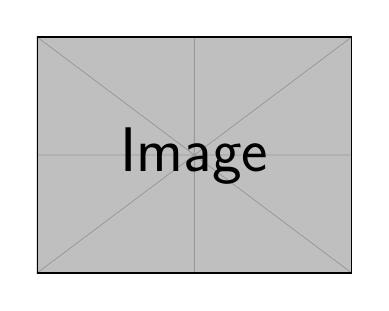
\begin{tikzpicture}
            \node at (0, 0) {\includegraphics[width=4cm]{example-image}};
        \end{tikzpicture}
    \end{center}\begin{solution}
    \begin{align*}
        \intertext{For the observer attached in the frame of disks}
        \mathbf{N} + \mathbf{F}_{\text{cor}} + mg + \mathbf{F}_{\text{cf}} &= 0 \tag{1} \\
        \text{So,} \quad \mathbf{N} &= -(\mathbf{F}_{\text{cor}} + mg + \mathbf{F}_{\text{cf}}) \tag{2} \\
        \text{So,} \quad |\mathbf{N}| &= \sqrt{(2m v' \omega)^2 + (mg)^2 + (m\omega^2 r)^2} \tag{3}
    \end{align*}
\end{solution}
    
\item Two solid bodies rotate about stationary mutually perpendicular intersecting axes with constant angular velocities \(\omega_1 = 3.0 \text{ rad/s}\) and \(\omega_2 = 4.0 \text{ rad/s}\). Find the angular velocity and angular acceleration of one body relative to the other.

\begin{solution}
    \begin{center}
        \begin{tikzpicture}
            \pic at (0, 0) {frame=3cm};
        \end{tikzpicture}
    \end{center}
    
    \begin{align*}
        \intertext{The angular velocity is a vector as infinitesimal rotation commute. As for relative linear velocity, the relative angular velocity of the body 1 with respect to the body 2 is clearly}
        \vec{\omega}_{12} &= \vec{\omega}_1 - \vec{\omega}_2\\
        \intertext{As $\vec{\omega}_1 \perp \vec{\omega}_2$, so, $|\vec{\omega}_{12}| = \sqrt{\omega_1^2 + \omega_2^2} = 5 \text{ rad/s}$ (on substituting values)}
        \intertext{If frame $K'$ rotates with angular velocity $\vec{\omega}$ with respect to frame $K$, the relation between the time derivatives of any vector $\vec{a}$, seen from different frames is:}
        \left.\dfrac{d \vec{a}}{dt}\right|_K &= \left.\dfrac{d \vec{a}}{dt}\right|_{K'} + \vec{\omega} \times \vec{a}
        \intertext{If frame attached with the intersection point of two axes (about which solids are rotating) is K and the frame attached with rotating solid with angular velocity $\vec{\omega}_2$ is $K'$}
        \text{Then,} \qquad \left.\dfrac{d \vec{\omega}_1}{dt}\right|_K &= \left.\dfrac{d \vec{\omega}_1}{dt}\right|_{K'} + \vec{\omega}_2 \times \vec{\omega}_1
        \intertext{However,} \qquad \left.\dfrac{d \vec{\omega}_1}{dt}\right|_K &=0 \quad \text{(as the first body rotates with constant angular velocity in space)}\\
        \text{and} \qquad \left.\dfrac{d \vec{\omega}_1}{dt}\right|_{K'} &= \vec{\beta}_{12} \quad \text{(the sought angular velocity)}\\
        \text{Hence,} \qquad \vec{\beta}_{12} &= \vec{\omega}_1 \times \vec{\omega}_2\\
        \text{So,} \qquad |\vec{\beta}_{12}| &= \omega_1 \omega_2 = 12 \text{ rad/s}^2 \quad \text{(on substituting values)}
    \end{align*}
\end{solution}

    \item A horizontal disc of radius \( R \) rotates with a constant angular velocity \( \omega \) about a stationary vertical axis passing through its edge. Along the circumference of the disc a particle of mass \( m \) moves with a velocity that is constant relative to the disc. At the moment when the particle is at the maximum distance from the rotation axis, the resultant of the inertial forces \( F_{in} \) acting on the particle in the reference frame fixed to the disc turns into zero. Find:
    \begin{enumerate}
        \item the acceleration \( w' \) of the particle relative to the disc;
        \item the dependence of \( F_{in} \) on the distance from the rotation axis.
    \end{enumerate}
    
\item A round cone with half-angle \( \alpha = 30^\circ \) and the radius of the base \( R = 5.0 \) cm rolls uniformly and without slipping over a horizontal plane as shown in Fig. 1.8. The cone apex is hinged at the point \( O \) which is on the same level with the point \( C \), the cone base centre. The velocity of point \( C \) is \( v = 10.0 \) cm/s. Find the moduli of
\begin{center}
    
\begin{tikzpicture}
        \node at (0, 0) {diagram.png};
    \end{tikzpicture}
\end{center}
\begin{enumerate}
    \item the vector of the angular velocity of the cone and the angle it forms with the vertical;
    \item the vector of the angular acceleration of the cone.
\end{enumerate}
    \item A train of mass \( m = 2000 \) tons moves in the latitude \( \varphi = 60^\circ \) North. Find:
    \begin{enumerate}
        \item the magnitude and direction of the lateral force that the train exerts on the rails if it moves along a meridian with a velocity \( v = 54 \) km per hour;
        \item in what direction and with what velocity the train should move for the resultant of the inertial forces acting on the train in the reference frame fixed to the Earth to be equal to zero.
    \end{enumerate}
  \end{enumerate}


\end{document}
